\documentclass{article}

\usepackage[a4paper,left=18mm,right=18mm,top=20mm,bottom=18mm]{geometry}
\usepackage[italian]{babel}

\usepackage{titling}
\usepackage{graphicx}
\usepackage{subcaption}
\usepackage{float}

\title{Architecture: overview of the documentation (sprint 1)}
\author{Nicolas Anselmi, David Guzman Piedrahita and Marco Vinciguerra}


\begin{document}
\maketitle

\section{Architecture design metod }
Per derivare una prima architettura funzionante partendo dai requirements specificati nell’apposito documento, si segue il criterio Generalized Model di Hofmeister et al. (2007).
\\Questo architecture design method è particolarmente utile per il progetto in questione, in quanto è strutturato utilizzando la terminologia e i ragionamenti di SCRUM, che è il life-cycle agile usato per l’applicazione e il suo sviluppo. 
\\In particolare, usa lo stesso concetto di backlog per elencare i diversi problemi che devono essere gestiti, e da esso è possibile scegliere gli elementi ritenuti più importanti in ogni particolare iterazione. 
\\Il backlog ha in input i requirements del progetto, con particolare attenzione ai requisiti di qualità; il contesto, che contiene idee aggiuntive sul come implementare un sistema che soddisfi i requisiti e, infine, i risultati della valutazione dell’architettura dell’iterazione precedente. 
\\Nel progetto verranno presi in considerazioni questi tre fattori per determinare le scelte di design. 
\\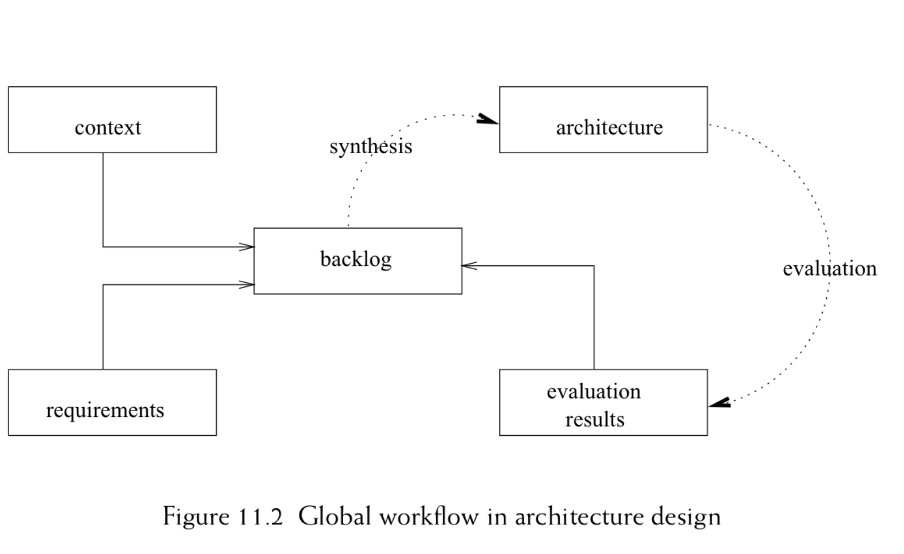
\includegraphics[scale = 0.75]{"Immagini/GeneralizedModel.png"}
\section{Decisioni di design} 
\subsection{Decision 1}
\begin{itemize}
\item Issue 
\item Decision
\item Status 
\item Assumptions
\item Alternatives
\item Rationale
\item Implications
\item Notes
\end{itemize}

\end{document}
